\documentclass[a4paper,11pt,pdf]{../templates/pacmanreport}

%%=== Aditional packages


%%=== Local definitions
\graphicspath{{images/}{../shared_images/}}

%% ================================
%% PROJECT INFO 

\project{}
\projectid{FP7-IST-60918}
\projectstart{1 March 2013}
\duration{36}

%% ================================
%% DELIVERABLE INFO 

\title{Bound compositional hierarchies modeling 2D and 3D visual shape of object categories}
\deliverableid{DR 1.3}
\author{M. Popa, J. L. Wyatt, A. Leonardis, D. Tabernik, V. Kramarev, R. Aktas, D. Belter, J. Piater, M. Ozay}
\address{Institute of Computer Science, University of Innsbruck}
\email{Mirela.Popa@uibk.ac.at}
\headertitle{Compositional Hierarchies}
\headerauthor{Popa et al.}

\duedate{2016-02-29}
\submissiondate{2016-02-29}
\leadpartner{UIBK}
\revision{draft}
\disseminationlevel{PU}


%% UNCOMMENT: to get the logo; if you've copied this file to a directory yearX/wpY/ then this should work
\reportlogo{pacmanlogo}


\begin{document}

\maketitle

\begin{abstract}
\noindent Compositional hierarchies are a particular form of representation for objects that we are investigating in the project. In this report we describe progress on several fronts regarding these hierarchies. We present, first of all, a method for learning compositional hierarchies that are linked across 2D intensity features and view based 3D depth features. We show that this is able to infer 3D object shape from 2D intensity edge information. Additionally we report several other advances we have made. These include several instantiations of our hierarchy that follow the same broad principles, and also the use of popular deep networks (CNNs) to perform similar tasks. The instantiations of our hierarchies include: a surface based version of our compositional hierarchy for modelling 3D shape; a mixed surface and volume based version of our hierarchy for the same purpose; and a 2D intensity version hierarchy for modelling of object appearance from edge images. We describe the general principles that we believe are essential for these hierarchies to work. These include: redundancy, generative modelling, and techniques for consistification. Our compositional hierarchical approach described here has been connected to the grasping algorithms developed previously, and this is described in DR2.2.
\end{abstract}


\vspace{.2em}
\hrule

\footnotesize

\tableofcontents

\normalsize

\newpage

\section*{Executive Summary}

%What does the report present? What tasks does it address? How has progress been evaluated? What previous reports does this report follow up on? 

In previous years the project peformed work on various extensions to a baseline compositional hierarchical approach. This included: i) adapting compositional hierarchical models developed for single viewpoint intensity images to multi-view recognition; ii) revision of the original model that was graph-theoretically sound; iii) a framework for compositional modelling from single view depth images. The focus in the final year has been on: i) learning linked compositional hierarchies; ii) learning view independent 3D hierarchies; iii) a probabilistic generative version of our 2D intensity based hierarchy; iv) investigations of alternative approaches such as CNNs. This report thus addresses all the remaining work done for tasks in WP1, especially Task 1.3. Progress has been evaluated by working on two common datasets that we have created: the PacMan grasping dataset used with our IJRR paper; and a new synthetic dataset of 400 objects with several hundred thousand depth and intensity images of those. We have also, where appropriate, used external datasets, such as CIFAR-10.

\section*{Role of Compositional Hierarchies in PaCMan}

%What role do the tasks addressed in this report play in the larger context of PaCMan? How do these tasks, how does report, contribute to achieving the overall goals for PaCMan? 
The work in WP1 is about developing models of object shape. The objective is to provide models of object appearance and shape that are robust to shape variability within categories, are compact, hierarchical, and robust to missing data. Finally the models should be of a form where they are suitable to support manipulation actions such as grasping. Thus this workpackage feeds into WP2, WP4, and WP5.

\section*{Contribution to the PaCMan scenario}

%How do the results presented in this report contribute to the PaCMan\cite{ProjectWebsite} scenarios and prototypes? 
The PacMan scenario is grasping and manipulation of unfamiliar objects. The results presented in this workpackage feed into work on grasping of unfamiliar objects described in WP2. They will also feed into one of the demonstrators in WP5.

\newpage

\section{Tasks, objectives, results}

\subsection{Planned work}

%What tasks was the report supposed to address? What objectives, results were these tasks to achieve? 
The main goal for the final stage of the project was to complete Task 1.3.
\begin{quotation}
{\em Task 1.3 Integration of 2D and 3D representations of objects:} We will integrate (bind) the two information channels, the one that models 2D shape fragments on various levels of complexity and the other that structures 3D elements in a compositional hierarchy. The integration will take a form of feature binding at various levels of granularity. We will learn significant statistical correlations between the two channels and link together the co-occuring features in a probabilistic sense.
\end{quotation}

For the final period the specific sub-goal was to ``Develop an efficient inference process that will operate both on combined (i.e., 2D
and 3D visual information channels) as well as on the individual ones.''

\subsection{Actual work performed}

%What does the report actually present? How have the tasks been addressed? To what extent have the intended objectives been achieved? Why, how -- or why not? 

We have achieved the goal of Task 1.3, using an approach based, as promised, on a pair of linked compositional hierarchies. Each hierarchy employs stacked autoencoders. The links between the 2D and 3D features are learned using the probabilistic approach to this that we presented at the Year 2 review. We also completed work on several instantiations of our compositional hierarchy that utilise the same core learning framework, but which have different ways of encoding object shape. The first encodes the 2D shape on the image plane caused by intensity changes. The second encodes the 3D shape of the object in a view based manner, expressing the changing depth of the object surfaces relative to the image plane. The third and fourth instantiations encode the 3D shape of the object in a view independent manner. The third instantiation does this in a surface based way, the fourth instantiation starts with this, and then builds on top of it a volumetric representation of 3D shape. In another WP we have combined this representation with our grasping algorithms. Finally, we have studied and implemented competing methods in the form of CNNs. In addition to all these pieces of work, we have generated a new dataset, containing 400 objects from 20 categories, which contains several hundred thousand depth and intensity images of these objects. We have used this for training of our compositional hierarchies. In addition it is intended for use as an enlarged training set for the cluttered scene challenge we presented as part of SHREC. Finally we participated in a workshop at ICCV, where we presented this challenge, and also a full ICCV paper on the theory of compositional hierarchies. The current work has resulted in drafts of three papers to be submitted to ECCV, and one paper to be submitted to IROS.

\subsubsection{Linked 2D-3D compositional hierarchies}

In a paper to be submitted to ECCV, and included in Annex A.1, we describe our proposed method for constructing two hierarchical representations, for two information channels, 2D intensity data and view-based 3D depth data. We employed as a learning algorithm a sparse autonencoder network, where each layer receives as input the latent representation of the layer below. For obtaining predictions across hierarchies, we discretized the responses of each layer into a set of parts, using clustering techniques. Furthermore, we introduced a probabilistic fusion model for linking the two information channels across hierarchies. The fused model enables an improved and refined representation of the world, while being able to infer 3D object shape from 2D intensity edge information.

Next, we evaluated the statistical relationship between representations obtained from 2D and view-based 3D models, analysis which facilitates also the understanding of the geometric properties of the two compositional representations. The evaluation of the learned correspondences between parts in the two hierarchies showed that meaningful correlations can be formed for a set of parts, while specific 2D parts have a high conditional entropy, due to ambiguity of edge structures which could correspond to many depth parts. We handled this problem, by extracting complementary information from the region surrounding an edge part using HOG features, which were fed to a SVM classifier. This method proved its usefulness in the inference process, leading to an improved detection of the correct corresponding depth part. The proposed approach and algorithms were examined on the PaCMan dataset. Experimental results show the efficacy of our approach for inferring view-based 3D information from observed 2D intensity data. 

\paragraph{Relation to SOTA:} 

The review of the works dealing with 2D and view-based 3D information showed that there are several approaches which tackle this problem using flat models, having a wide range of applications. Face recognition is investigated by Arca et al.~\cite{Arca2007} by fusing the two modalities at an early stage and by Soltana et al.~\cite{Soltana2010} who propose a fusing strategy consisting of an offline and an online weight learning process. 3D object retrieval based on a 2D image is investigated by Eitz et al.~\cite{Eitz2012} using a sketch representation based on optimized Gabor filters, followed by a bag-of-words approach. 2D-to-3D movie conversion was addressed by Cheng et al.~\cite{Cheng2010}, using the assumption that edge information in an image has a high probability of also being an edge in the depth map.
Recovering 3D depth from a single image for scene understanding represents an important topic in computer vision and was investigated by Tian et al.~\cite{Tian2014} using a deep learning model, by Saxena et al.~\cite{Saxena2009} by means of a Markov Random Field(MRF) model which captured the relationships between different parts of an image and by Konrad et al.~\cite{Konrad2012} who proposed a depth sampling method, by fusing the corresponding depth images of the top $k$-nearest neighbour images of the query image.
An approach similar to ours was proposed by Masci et al.~\cite{Masci2011}, where stacked autoencoders are trained in a similar fashion, while the main novelty addressed in our work, is the cross-hierarchy prediction power which facilitates view-based 3D inference from observed 2D intensity data.

\subsubsection{2D intensity-based compositional hierarchies}

In this line of work we have been refining work on compositional hierarchies through our graph theoretically grounded CHOP algorithm. This was published in ICCV 2015. This addresses the problem of learning shape models that are invariant to translations, rotations, and scaling. We address this particularly for the case of shapes that have multiple disconnected components. Moving beyond CHOP we have attempted to build a hierarchy that is probabilistically clean, and which attempts to maximise data likelihood. This has led to a new formulation that we will present at the review. In addition we have investigated what can be done with CNNs. In particular we have looked at how to simplify CNNs by constraining weights in the network to lie on a Gaussian. Our early experiments, which have been drafted into a paper to be submitted to ICPR, show that this does not affect the quality of learning. 

\paragraph{Relation to SOTA:} 

Our work is inspired by evidence that visual data processing in the brain is hierarchical, consisting of multiple layers responsible for different complexity classes \cite{report:kruger}. Many hierarchical vision algorithms that imitate this type of behaviour \cite{rev1} have been developed. These require tractable layer-wise learning and part shareability. However, the optimization functions for part selection depend on the task. Hierarchical dictionaries have been trained for object categorization \cite{report:shen,fidler_cvpr07}, recognition \cite{report:recognition} and detection \cite{felz,report:kokkinos,girshick2014rcnn} problems. 

Convolutional Neural Networks (CNNs) \cite{Lenet} are an alternative to compositional hierarchies that have shown excellent performance on vision-related tasks. Their resurgence can be attributed to Krizhevsky et al. \cite{Krizhevsky} achieving state-of-the-art performance in ILSVRC-2012, on the ImageNet classification task. Powerful computers and large datasets have been critical in this advance, as evident in a 150-layer network by He et al. \cite{DBLP:journals/corr/HeZRS15} winning the ILSVRC-2015 and COCO-2015 competitions. A difference between our approach and deep networks is that most of the compositional hierarchies that we study perform local function approximation at each layer, rather than the global transformations performed in CNNs, although we have moved in the direction of global function approximation with our other work on stacked auto-encoders. 

Local function approximation generally produces more human understandable representations, and this may be seen as an advantage of the line we are pursuing. Despite this recent papers on deep nets \cite{deepvis,Simonyan14a,DBLP:journals/corr/MahendranV15,deepvis2} have attempted to visualise learned representations for better understanding of the algorithms. Zeiler and Fergus \cite{deepvis}, for example, have demonstrated that CNNs are able to learn visually meaningful features. 

We are also pursuing work on using compositional hierarchies as generative models. In parallel there is work on this in deep networks. Simonyan et al. \cite{Simonyan14a}, for example, developed a method to generate a single image that is the representative of a class via gradient-based optimization of class scores. Also, true generative approaches for feature visualization have been developed for CNNs. Dai and Wu \cite{DBLP:journals/corr/DaiW14} perform generative sampling from discriminatively-learned deep neural networks. The generative gradient that minimizes reconstruction error is used in pre-training and visualisation. Similarly, Dosovitskiy et al. \cite{DB15} have presented a method that can generate previously unseen samples of a class (chairs) using CNNs. Overall, it is not yet entirely clear what the precise performance advantages of our approach versus CNNs is, although recent work by Hinton on capsules claims key deficiencies in CNNs with respect to spatial transformations---such as those handled well by our ICCV paper---and proposes mechanisms essentially similiar to those we are pursuing. This suggests that our approach, and hybrid approaches hold promise.

Our work on Compositional Hierarchy of Parts (CHOP) \cite{chop,CHOPManifold}, also has similarities with two previous hierarchical compositional frameworks, Learned Hierarchy of Parts (LHOP) by Fidler et al. \cite{fidler_cvpr07,lhop_book} and And-Or graphs by Si and Zhu \cite{report:SCZhu}. All three algorithms use simple features as low-level features, and learn compositional representations in the form of And-nodes, while articulations of a part are encoded in Or-nodes. 

\subsubsection{3D view invariant compositional hierarchies}

We have also been pursuing work on 3D compositional hierarchies. In previous years we developed a method that built 2.5D parts. This year we have moved to view independent 3D representations. We have explored two ways of growing the receptive fields of the parts. The first is essentially surface based, so that the receptive fields grow geodesically across the object's surface. The second is surface based at the lower levels, but at the higher levels it moves to a volumetric representation. At the moment we are able to show that both these 3D representations have the shareability property that is essential to scaling. We are currently evaluating both of these 3D representations, and we have linked one of them to our work on grasp learning using probabilistic representations.

\paragraph{Relation to SOTA:}  

Relatively little work has been done in the domain of 3D compositional part-based models. The classical work of Biederman was done in the 1980s \cite{biederman1987recognition}. In his approach geons are based on a set of standard geometric primitives (e.g. cylinders, cones), which are assembled to form object and category models. There exist several more recent methods in this domain. Wessel and Klein \cite{pratikakis2010learning}, for example, presented a feature selection technique, which decomposes 3D objects into sections that can be represented by planes, spheres, cylinders, cones and tori. They introduced a probabilistic framework modeling the spatial arrangements between these shape primitives. This early work \cite{biederman1987recognition,pratikakis2010learning} used a set of pre-defined shapes as simple primitives with very shallow hierarchical structures, which makes it difficult to generalise over complex shapes. In contrast, our methodology is entirely data-driven, and is able to learn structures of arbitrary size and complexity. 

More recently, neural networks have been used in creating 3D representations \cite{wu20153d,Su_2015_ICCV}. Wu et al. \cite{wu20153d} proposed a 3D hierarchical compositional framework called 3D-ShapeNet. They present a 3D model
as a probability distribution of binary variables on a 3D voxel grid, using a convolutional Deep Belief Network (DBN). They demonstrated the ability of their approach to recognize object categories from range images and complete full 3D shape of objects. Similarly, Su et al. \cite{Su_2015_ICCV} have applied convolution neural networks to the 3D shape recognition problem. They first perform recognition of objects presented from a single view, and then present a novel
CNN architecture that combines information from multiple views of each object into a single compact descriptor. Our method can be seen as an alternative based on local function approximation in each layer, as opposed to global function approximation. Local function approximators have quite different properties to global function approximators, producing more easily understandable features, and having different properties in terms of learning complexity.

Hu and Zhu \cite{hu2015learning} presented a framework for learning of 3D templates from 3D models of cars using AND-OR trees. They used the learned templates for simultaneous object detection, localization and pose estimation. This method exploits the well-defined 3D structure of cars to learn 3D compositions, which would otherwise be a combinatorial problem. It requires manual annotation of object parts, however, hence addition of new categories is difficult. Our approach does not require annotation of object parts, and is able to find recurring patterns in data automatically. Finally, methods based on deep learning \cite{wu20153d,Su_2015_ICCV} perform well on object categorization tasks. The challenge lies in designing the network to different tasks, since it is not possible to visualise the learned features in order to check if they are visually meaningful. 

\subsubsection{New PacMan dataset}

To support the work we have done on other aspects, we have employed a new dataset. This is a synthetic dataset, designed to give us clean data for learning, and also to enable the generation of a large number of views of common objects. This we refer to as the PaCMan Shape Dataset. It comprises a total of 400 objects across 20 categories, each having 20 models. The categories are all household objects, most of which are typical kitchen objects: mug, cup, fork, jug, plate, bowl, frying pan, tray, teapot, tea cup, cutting board, box, knife, vase, can, fork, spatula, scissors, bottle and shaker. The objects have realistic sizes, and their longest dimension ranges from 80 mm to 200 mm, depending on the category. One representative image out of every class is depicted in Fig. \ref{shapes}.

 \begin{figure}[!h]
  \caption{Representative shapes for every class in the dataset.}
  \centering
    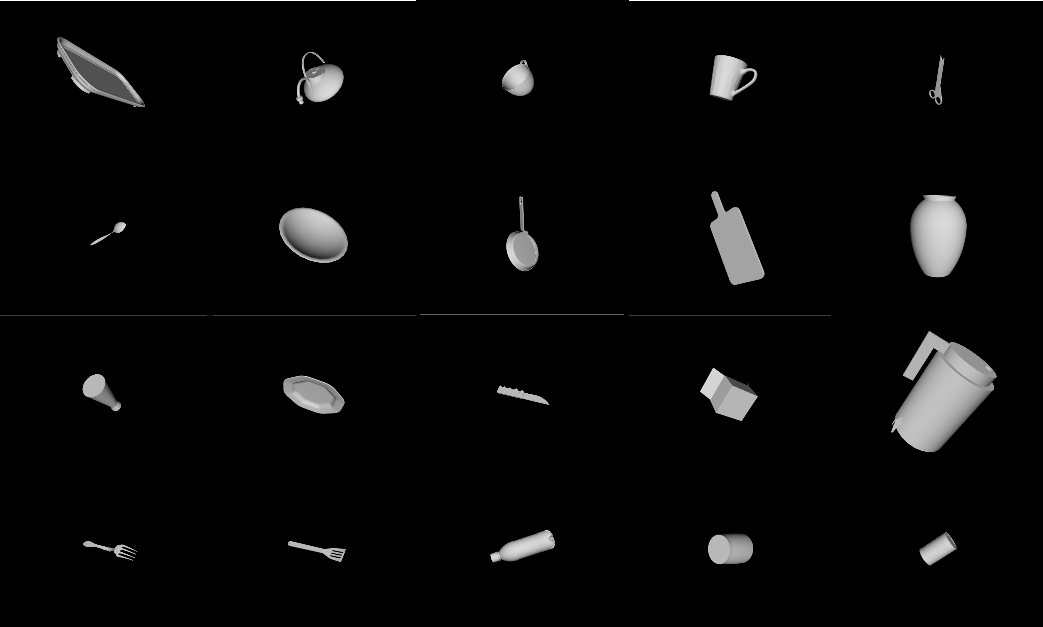
\includegraphics[width=\textwidth]{shapes.png}
\label{shapes}
\end{figure}

In order to render the objects from multiple viewpoints, we used 32 uniformly sampled points on the view sphere. The azimuth and elevation of these samples are given below. Fig \ref{viewSphere} shows the triangulation of the view sphere, where every vertex corresponds to a camera position, with the viewing vector directed to the centre of the sphere. We have  rendered every object from each viewpoint using a simulated RGB camera and a depth camera, which has the characteristics of a Carmine 1.09 sensor.
 
 
\begin{itemize}
\item azimuth =(358, 62, 238, 272, 195, 167, 274, 50, 230, 242, 273, 92, 347, 314, 58, 134, 297, 336, 94, 308, 93, 254, 178, 156, 26, 184, 206, 4, 15, 128, 74, 117)
\item elevation = (58, -38, -2, -26, -18, 12, -68, 39, -39, 38, 12, 26, -12, -38, 2, 38, 42, 24, 68, -1, -12, 75, -58, -24, -17, 50, 17, 50, 18, 1, -75, -42)
\end{itemize}

\begin{figure}[!h]
  \caption{View sphere triangulation.}
  \centering
    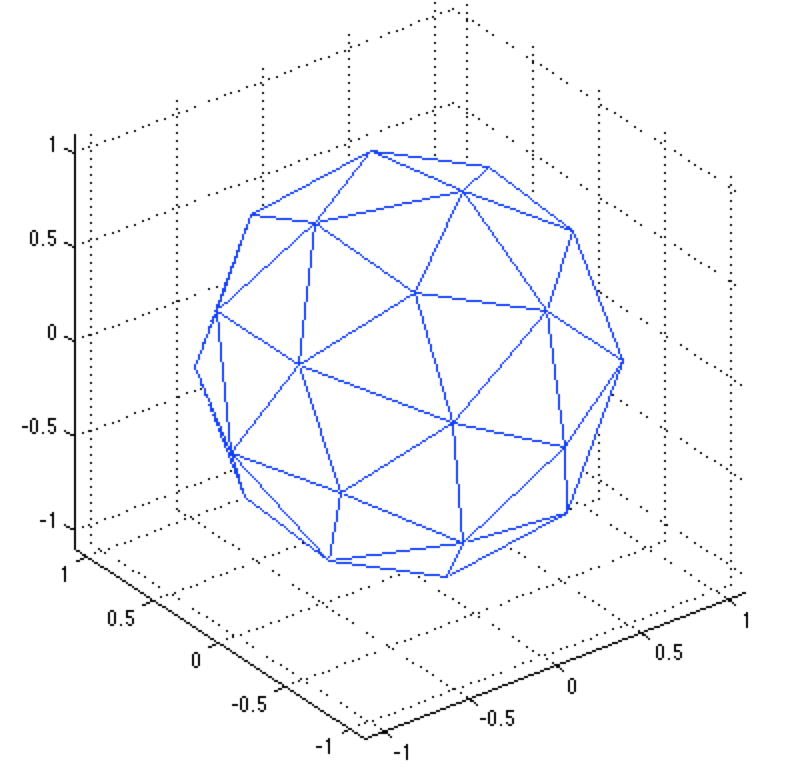
\includegraphics[width=0.6\textwidth]{viewSphere.png}
\label{viewSphere}
\end{figure}

The image acquisition process proceeded as follows:
\begin{enumerate}
\item The object was placed such that its centre of gravity is at the origin.
\item The camera was located on the y axis in various distances from the origin, namely, [0, 600mm, 0] or [0, 900mm, 0] or [0, 1200mm, 0].
\item Two light sources were placed in the scene. The more powerful light source was located above the camera, while the weaker one was below the camera, with respect to the camera's up vector. This created enough intensity differences to reveal intensity edges on the object. 
\item The camera was directed towards the origin. The camera had a horizontal Field of View of 57.5 degrees.
\item The near range of the camera was 350mm, and the far range was 1400mm. That meant that depth values in the range from 350mm to 1400mm were encoded in 2 byte values. Larger values correspond to closer distances.
\end{enumerate}

Rendered images of the objects in the dataset are placed in a hierarchical structure, and named in a specific way. For example, for a rendered image that has the name ``3\_P2\_IP3.png":
\begin{itemize}
\item 3 is the id of the object in the dataset (from 1 to 400)
\item P2 - that means that values a(2) and b(2) were used to rotate the object (we rotate the object, not the camera).
\item IP3 - id of the in-plane rotation. There are 8 IDs in total, describing 8 different angles of rotation of the camera about the y-axis, with a step size of 45 degrees. IP1, the initial configuration of the camera, corresponds to a zero degree rotation of the camera.
\end{itemize}

The category labels are stored in a 400x1 array that contains the label of every model in the dataset, distributed along with the images. The dataset is currently available at the following location:  \\

{\tt \small https://www.dropbox.com/s/9ti5mdkx4jcdlvg/400Pacmans.tar.gz?dl=0} 

\bibliographystyle{IEEEtran}
\bibliography{../shared_bibliography/abbreviations,./bibliography/DR13,egbib_rusen,inputFiles/KramarevECCV2016/refs}

\newpage

\appendix
\section{Annexes}

%Which papers / articles are included in the report? Mention titles, authors, publication info; abstract; and a one-liner relating the publication back to the discussion on actual work performed. 

% template for annexes
\subsection{Article: \em Hierarchical Object Representation based on a Sparse Autoencoder Network}
\begin{description}
    \item[Authors] Mirela Popa, Jeremy L Wyatt and Justus Piater
    \item[Info] This is a long version of a paper to be submitted to ECCV 2016.
    \item[Abstract] We propose a method for constructing a pair of complementary
hierarchical representations from 2D edge images and from view-based 3D
data, respectively.  As a learning algorithm, our model uses a sparse
autoencoder network, which propagates information bottom-up, while
offering an efficient inference mechanism across hierarchies, based on
discretization of the responses at each layer.  We introduce a
probabilistic fusion model for inferring missing observations across
modalities and for scene reconstruction by exploiting correlations
between 2D and view-based 3D observations. The results obtained on the
PaCMan dataset demonstrate the efficacy of our approach.
    \item [Relation with the deliverable] This work is concerned with learning and inference using a pair of linked 2D-3D hierarchies. This is one of primary goals of the WP, and the primary goal of Task 1.3. The paper describes how we create a compositional hierarchy using a stacked autoencoder. It then shows how we learn a pair of such hierarchies, one for 2D intensity information, and one for view based 3D information. The hierarchies are grown using the same principles we have developed elsewhere, including We then show how these hierarchies can be linked using probabilistically correct inference. Finally we show that this enables us to infer 3D structure from 2D intensity edges. This meets the goal of Task 1.3.
    
    \item[Attachment] The attachment is included at the end of the deliverable.
\end{description}
% attach your PDF(s) if required, pusblished and online available documents do not require it if you provide the doi (only doi are permitted)
%\includepdf[pages=-]{./attachedPapers/YOURFILE.pdf
\newpage

\subsection{Article: \em A view-invariant, compositional hierarchical representation of 3D shapes}
\begin{description}
    \item[Authors] Vladislav Kramarev, Ales Leonardis and Jeremy L. Wyatt
    \item[Info] To be submitted to ECCV 2016.
    \item[Abstract] We propose a novel, view-invariant, compositional hierarchical representation of 3D shape. The representation is surface based. The hierarchy is learned from 3D models, either point cloud or mesh data. The hierarchy is built in layers, where each layer is a vocabulary of parts, each part corresponding to some 3D surface. The parts in a layer are learned by composing parts from the layer below. The implementation of the framework allows learning of compact hierarchies. Each part is able to capture variation in shape, and does so by encoding densities over transformations between part poses, and measures of surface similiarity. Compactness is also achieved by the fact that the parts learned are shared across different object categories. In empirical work we show the features that the hierarchy learns, and demonstrate their shareability. Receptive fields for each layer are redundant, and grow geodesically across the surface of the object.
    \item [Relation with the deliverable] This paper describes a more advanced form of the previously view variant 3D compositional hierarchy that we presented in previous years. We have now moved this hierarchy to be completely view independent. This enables the parts to grow without restrictions imposed by the viewpoint. We demonstrate the learning on a PacMan dataset gathered specifically for this purpose. This work represents part of the progress we have made on compositional hierarchies for 3D shape.
    \item[Attachment] The attachment is included at the end of the deliverable. %if so, e.g. (following pages until next annex) or The article can be downloaded at the DOI link above, hence no attachment is provided
\end{description}
\newpage

\subsection{Article: \em Learning and inference with a compositional hierarchical representation
of 3D object shape}
\begin{description}
    \item[Authors] Domink Belter, Marek Kopicki, Ales Leonardis and Jeremy L. Wyatt
    \item[Info] To be submitted to IROS 2016. % UNDER REVIEW / IN PRESS / ACCEPTED FOR PUBLICATION (PROVIDE WHERE) / PUBLISHED AND AVAILABLE ONLINE (PROVIDE DOI)
    \item[Abstract] Modelling of object shape is an essential precursor to any method for object manipulation. In this paper
we present a method for learning compositional hierarchical representations of 2.5D and 3D object shape. These are representations
that consist of a hierarchy of parts. We present novel algorithms for learning and inference. We empirically demonstrate the ability to learn these representations from real
depth data, and to fill in missing information caused by self-occlusions. We also demonstrate the ability of the hierarchy to model variable shape, and to share parts across different
objects and object categories.
    \item [Relation with the deliverable] This paper describes an extension of the type of approach in the previous attachment. This compositional hierarchy starts with learning view invariant surface parts from viewpoint specific data. It then performs a further abstraction by creating parts that are based on volumetric receptive fields, and learned from data obtained from several different views. The hierarchy is the part of our work on 3D compositions that has been implemented to connect with our grasp learning algorithms. In this paper we describe how the hierarchy is learned, and show that it has the properties of view invariance, shareability and robustness to noise that we desire. To show the ability to learn in the face of noisy data we demonstrate learning on the IJRR dataset that 
    \item[Attachment] The attachment is included at the end of the deliverable. %if so, e.g. (following pages until next annex) or The article can be downloaded at the DOI link above, hence no attachment is provided
\end{description}
\newpage

\subsection{Article: \em Gaussian parametrization of deep convolutional network filters}
\begin{description}
    \item[Authors] Domen Tabernik and Ales Leonardis
    \item[Info] To be submitted to ICPR 2016% UNDER REVIEW / IN PRESS / ACCEPTED FOR PUBLICATION (PROVIDE WHERE) / PUBLISHED AND AVAILABLE ONLINE (PROVIDE DOI)
    \item[Abstract] In this work we propose to extend convolutional neural networks with an explicit spatial structure. We introduce
a restriction between a feature and its sub-features by explicitly incorporating a spatial relationship between them to represent
the spatial structure within object’s hierarchy. By proposing to model this relationship with Gaussian distributions we effectively
introduce a parametrization of CNN filters using a mixture of Gaussian distributions. We show how parametrization can fit
into the learning with back-propagation and gradient descent, and further show that standard convolutional neural network
can be considered as a special case of the proposed model. More importantly, we show that proposed model can now be
considered as composition hierarchy, thus opening a way to incorporate generative properties of compositional hierarchies
in the future. This work focuses on analyzing the viability of proposed model by evaluating it on a simple synthetic case and on
two classification dataset, CIFAR-10 and PaCMan database. We show that proposed model achieves the same level of performance
as standard CNNs, but achieves higher level of compactness of filters and is a first step towards the compositional interpretation
of the representation being learned through CNNs.
    \item [Relation with the deliverable] This paper describes work on applying CNNs to learning object categories. The study looks at the performance of a CNN implementation on two datasets CIFAR-10 and the PacMan synthetic object dataset. The paper focuses on 2D intensity images, and on object categorisation. Part of the purpose of this investigation was to assess the level of performance of CNNs on similar data to that used by our compositional hierarchies. The paper looks at ways of simplifying CNNs while retaining their performance, the approach being to constrain weights to lie on a Gaussian. 
    \item[Attachment] The attachment is included at the end of the deliverable. %if so, e.g. (following pages until next annex) or The article can be downloaded at the DOI link above, hence no attachment is provided
\end{description}
\newpage


\subsection{Article: \em Compositional Hierarchical Representation of Shape Manifolds for Classification
of Non-manifold Shapes}
\begin{description}
    \item[Authors] Mete Ozay, Rusen Aktas, Jeremy L. Wyatt and Ales Leonardis
    \item[Info] Published in ICCV 2015 % UNDER REVIEW / IN PRESS / ACCEPTED FOR PUBLICATION (PROVIDE WHERE) / PUBLISHED AND AVAILABLE ONLINE (PROVIDE DOI)
    \item[Abstract] We address the problem of statistical learning of shape models which are invariant to translation, rotation and scale in compositional hierarchies when data spaces of measurements and shape spaces are not topological manifolds. In practice, this problem is observed while modeling shapes having multiple disconnected components, e.g.
partially occluded shapes in cluttered scenes. We resolve the aforementioned problem by first reformulating the relationship between data and shape spaces considering the interaction between Receptive Fields (RFs) and Shape Manifolds (SMs) in a compositional hierarchical shape vocabulary. Then, we suggest a method to model the topological
structure of the SMs for statistical learning of the geometric transformations of the shapes that are defined by group
actions on the SMs. For this purpose, we design a disjoint union topology using an indexing mechanism for the formation of shape models on SMs in the vocabulary, recursively. We represent the topological relationship between
shape components using graphs, which are aggregated to construct a hierarchical graph structure for the shape vocabulary. To this end, we introduce a framework to implement the indexing mechanisms for the employment of the vocabulary for structural shape classification. The proposed approach is used to construct invariant shape representations. Results on benchmark shape classification outperform state-of-the-art methods.
\item [Relation with the deliverable] This shows the completion of our work on CHOP, and the ability of the CHOP method to draw inferences in the face of occlusions.
\item[Attachment] The attachment is included at the end of the deliverable. %if so, e.g. (following pages until next annex) or The article can be downloaded at the DOI link above, hence no attachment is provided
\end{description}
\newpage

%
%\subsection{Article: \em A probabilistic generative compositional hierarchy for modelling 2D object shape}
%\begin{description}
%    \item[Authors] Rusen Aktas, Ales Leonardis and Jeremy L. Wyatt
%    \item[Info] To be submitted to ECCV 2016 % UNDER REVIEW / IN PRESS / ACCEPTED FOR PUBLICATION (PROVIDE WHERE) / PUBLISHED AND AVAILABLE ONLINE (PROVIDE DOI)
%    \item[Abstract] 
%    \item [Relation with the deliverable] This paper is the conclusion of our work on compositional hierarchies for 2D intensity images. As in the first two years of the project we learn the hierarchy from multiple views, using edge features extracted from intensity images. At the start of the project the LHOP approach was used. Following this we developed CHOP. The purpose of CHOP was to provide a theoretically sound way (MDL) to trade-off the description length of the parts against their explanatory power. This was done with a graph theoretic approach. In this final iteration we have also made the formulation better grounded in terms of probability theory. This has been achieved by using a generative compositional hierarchical model. The generative model allows us to sample images from nodes at higher layers in the hierarchy. This is achieved using a stochastic grammar, a product of experts, and an optimisation procedure for maximising the likelihood of generated images. This allows us to achieve one of the goals of the hierarchy, which is to run it as a generative model, thus showing the ability to fill in missing data.
%    
%    \item[Attachment] The attachment is included at the end of the deliverable. %if so, e.g. (following pages until next annex) or The article can be downloaded at the DOI link above, hence no attachment is provided
%\end{description}
%\newpage

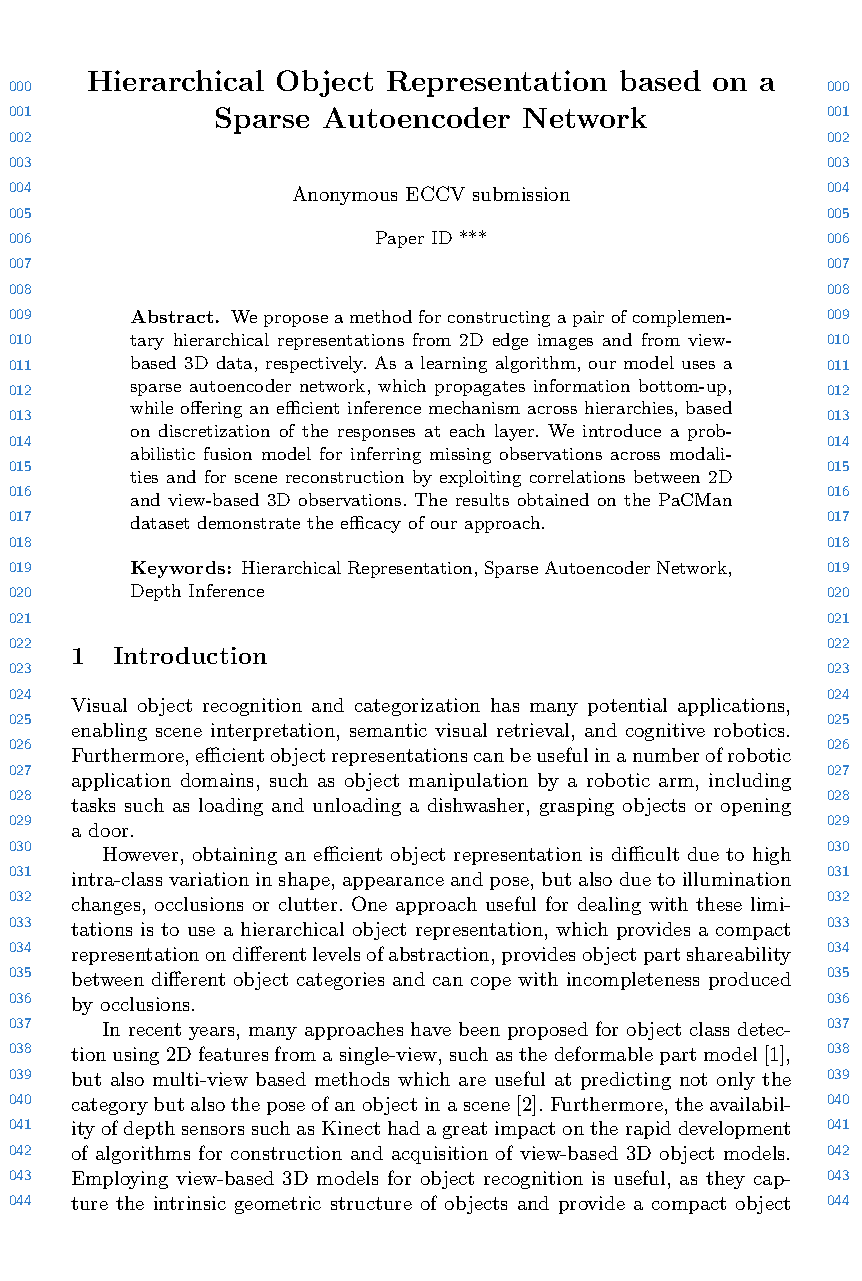
\includepdf[pages=-]{./attachedPapers/HierarchicalSparseAutoencoders.pdf}

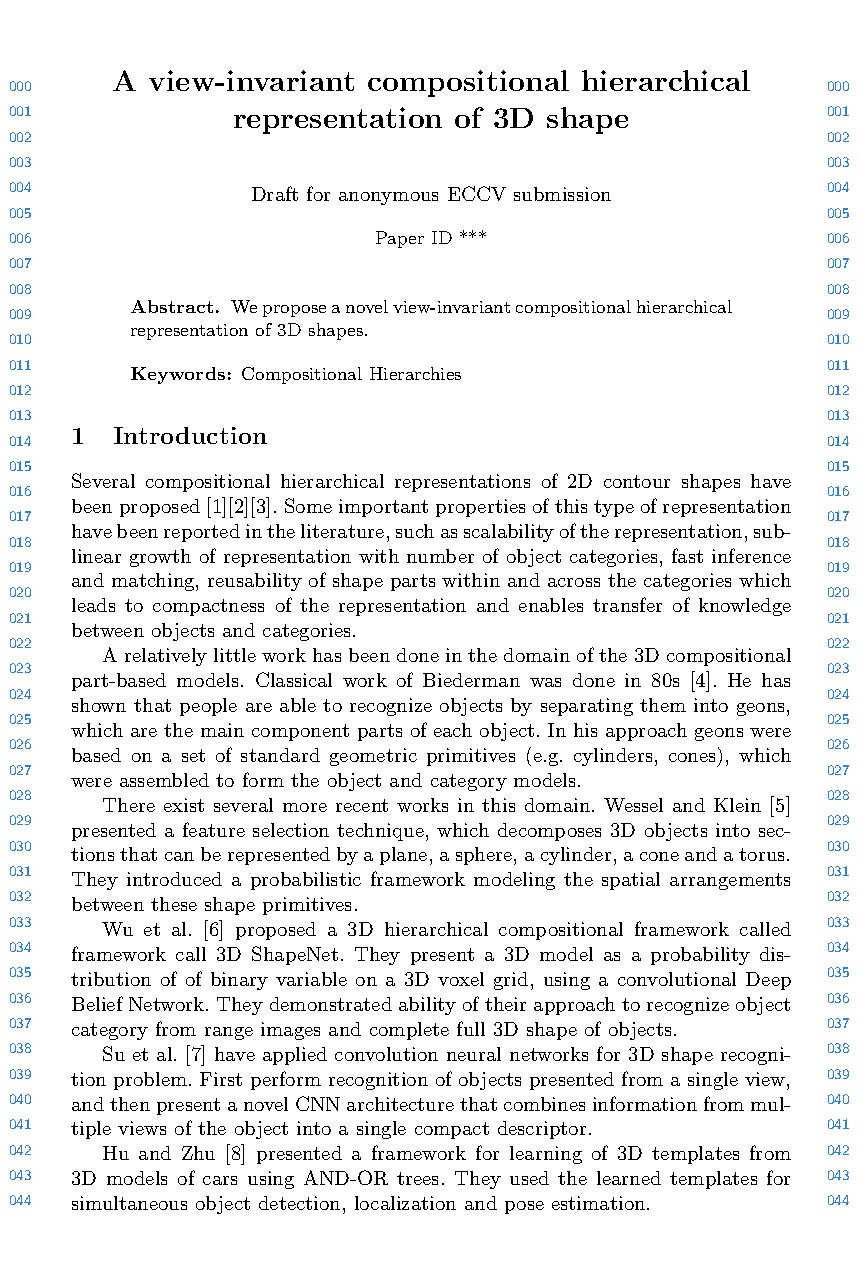
\includepdf[pages=-]{./attachedPapers/eccv2016submission.pdf}

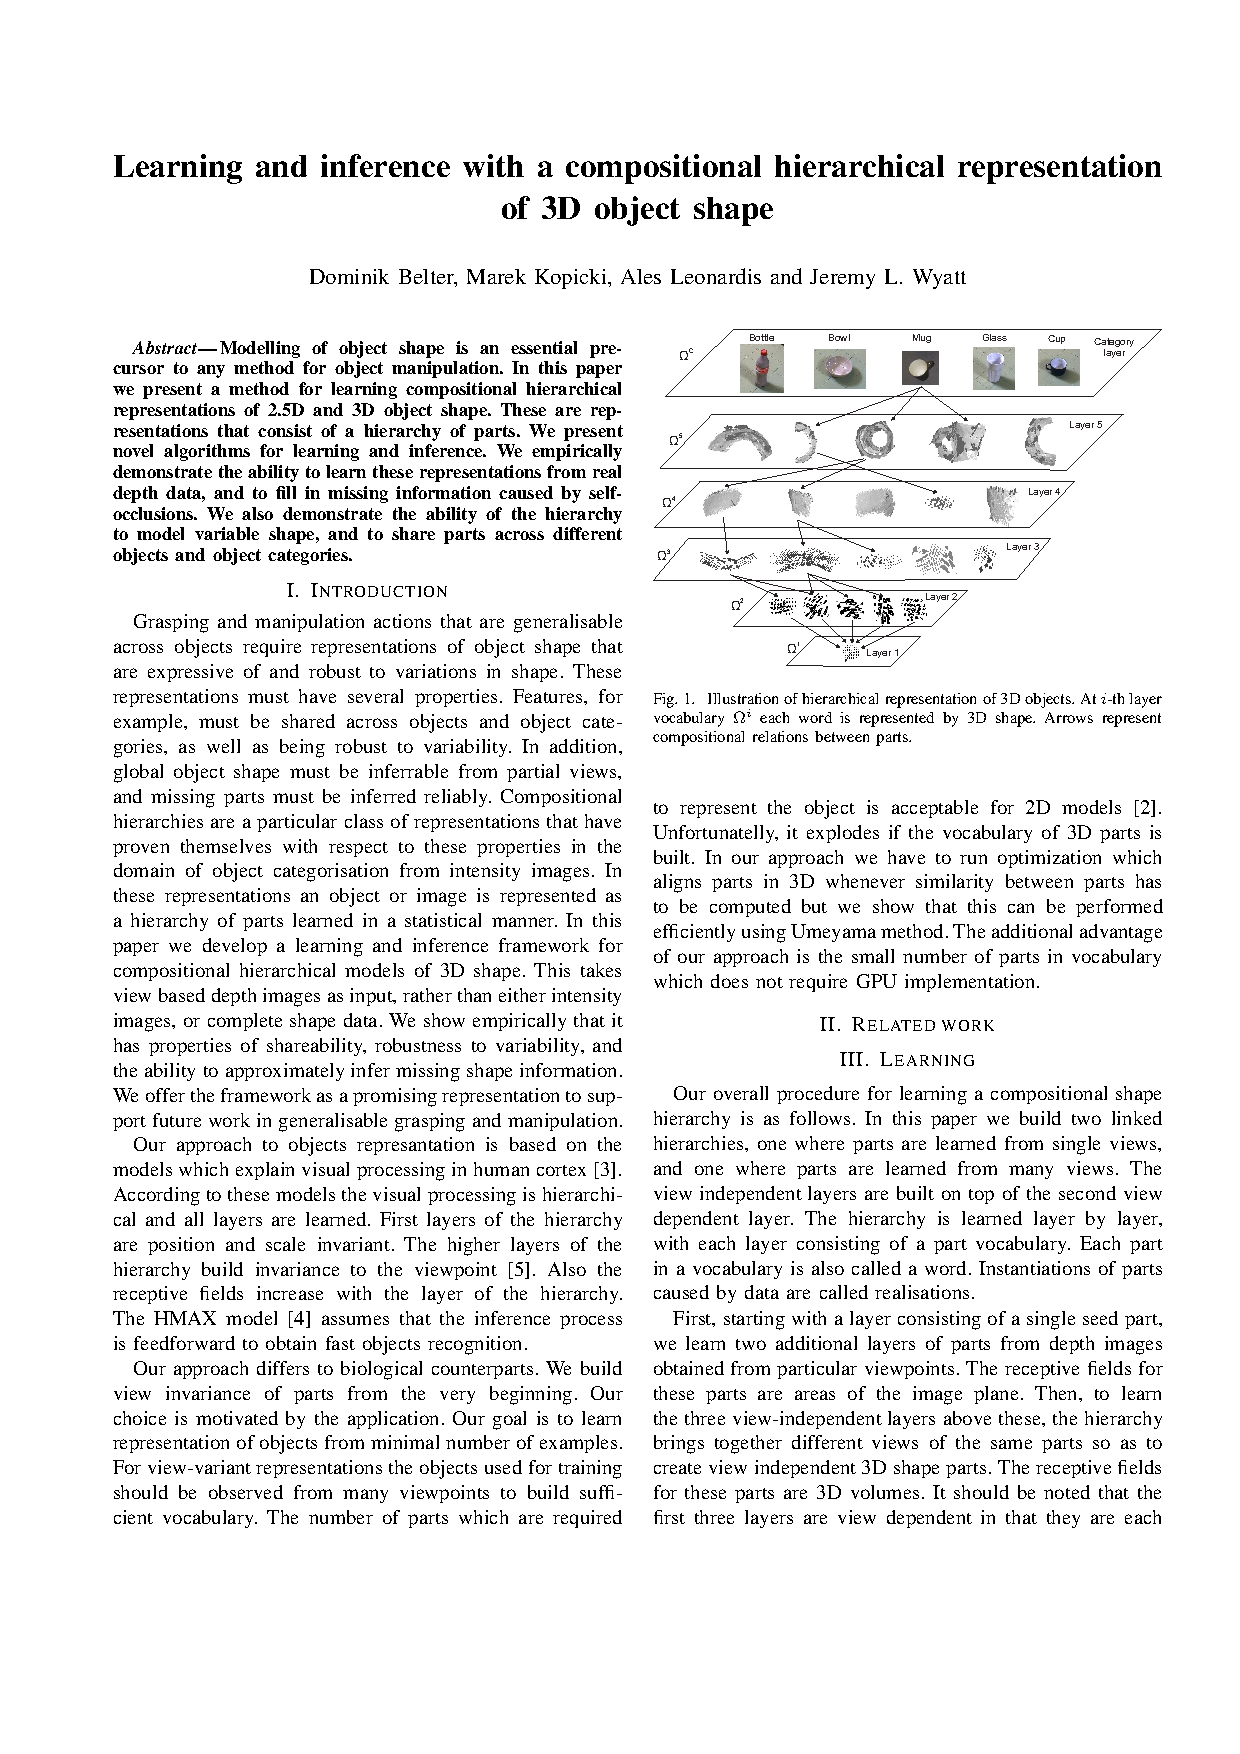
\includepdf[pages=-]{./attachedPapers/finalReport.pdf}

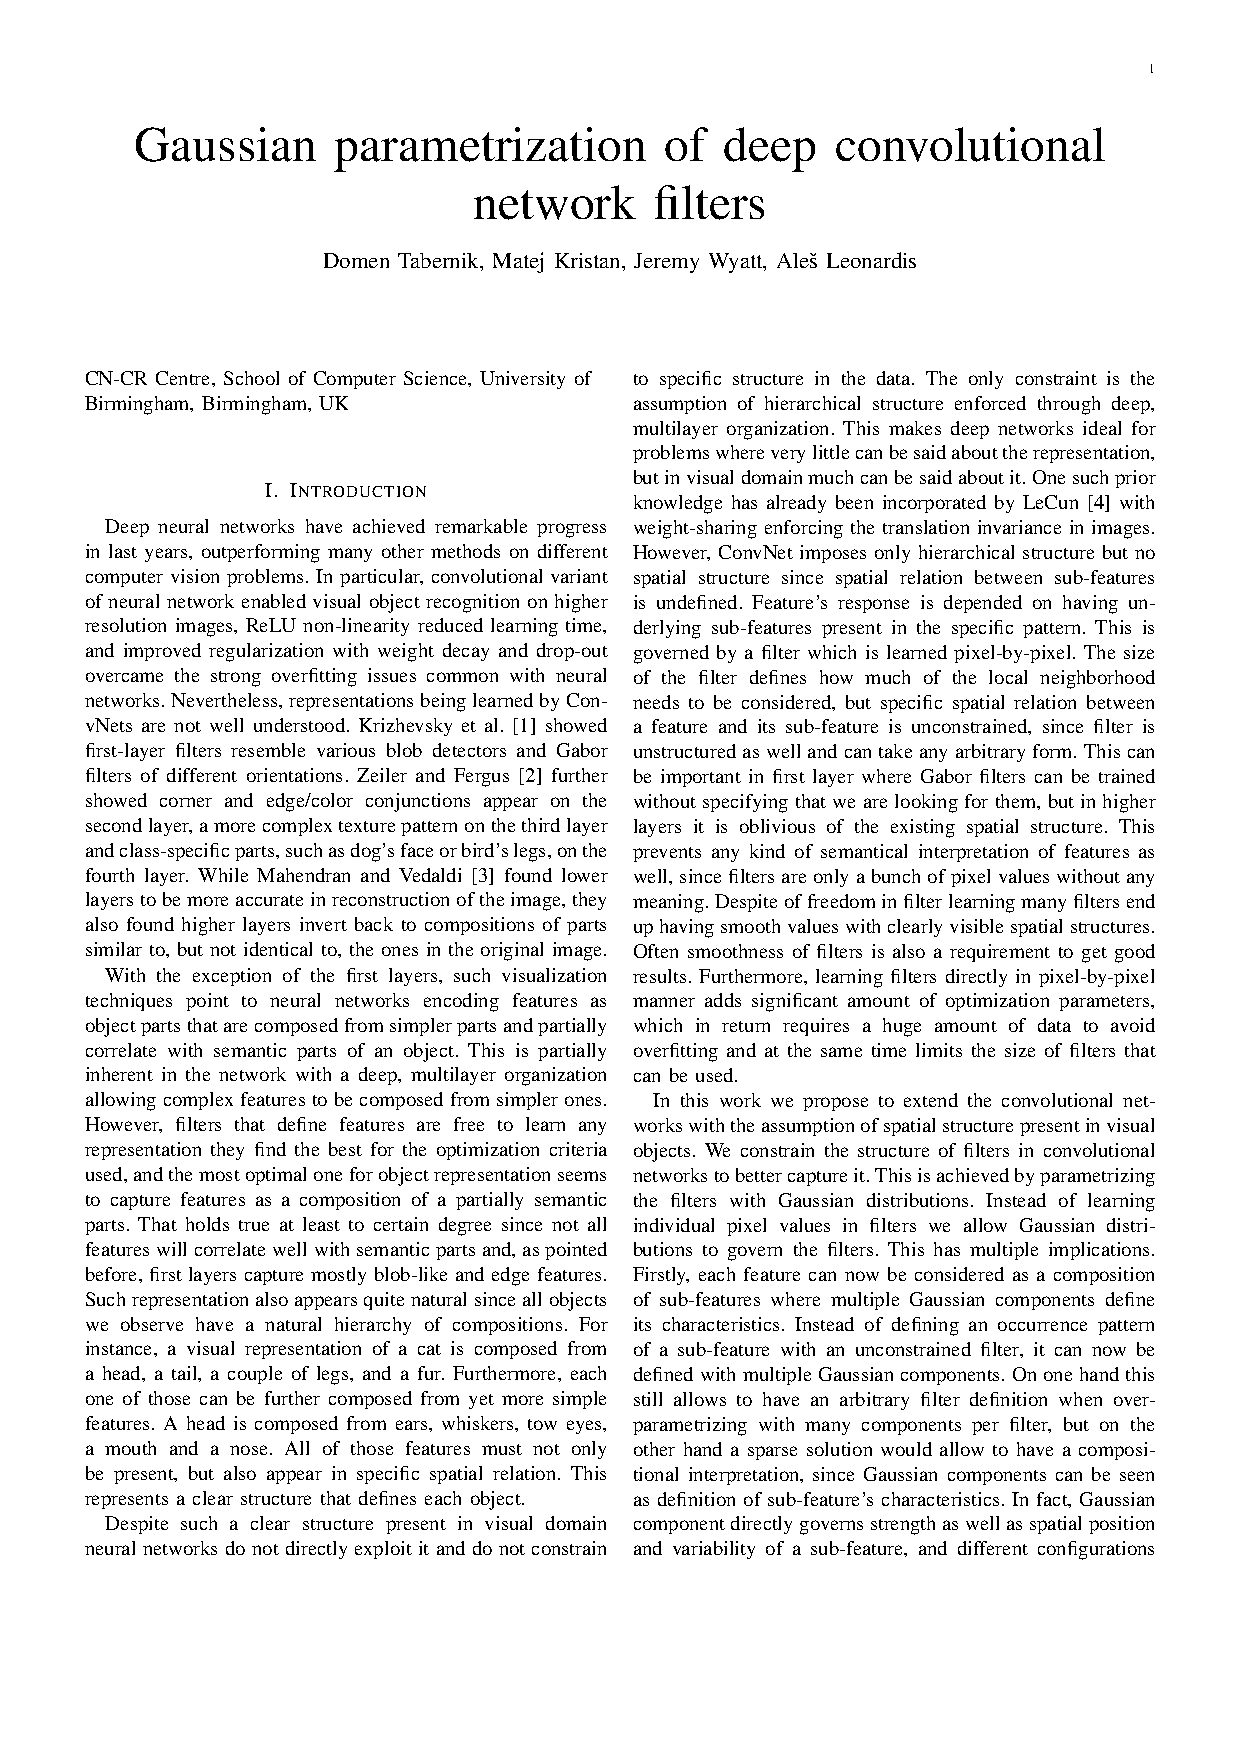
\includepdf[pages=-]{./attachedPapers/GaussianCNN_TechReport.pdf}

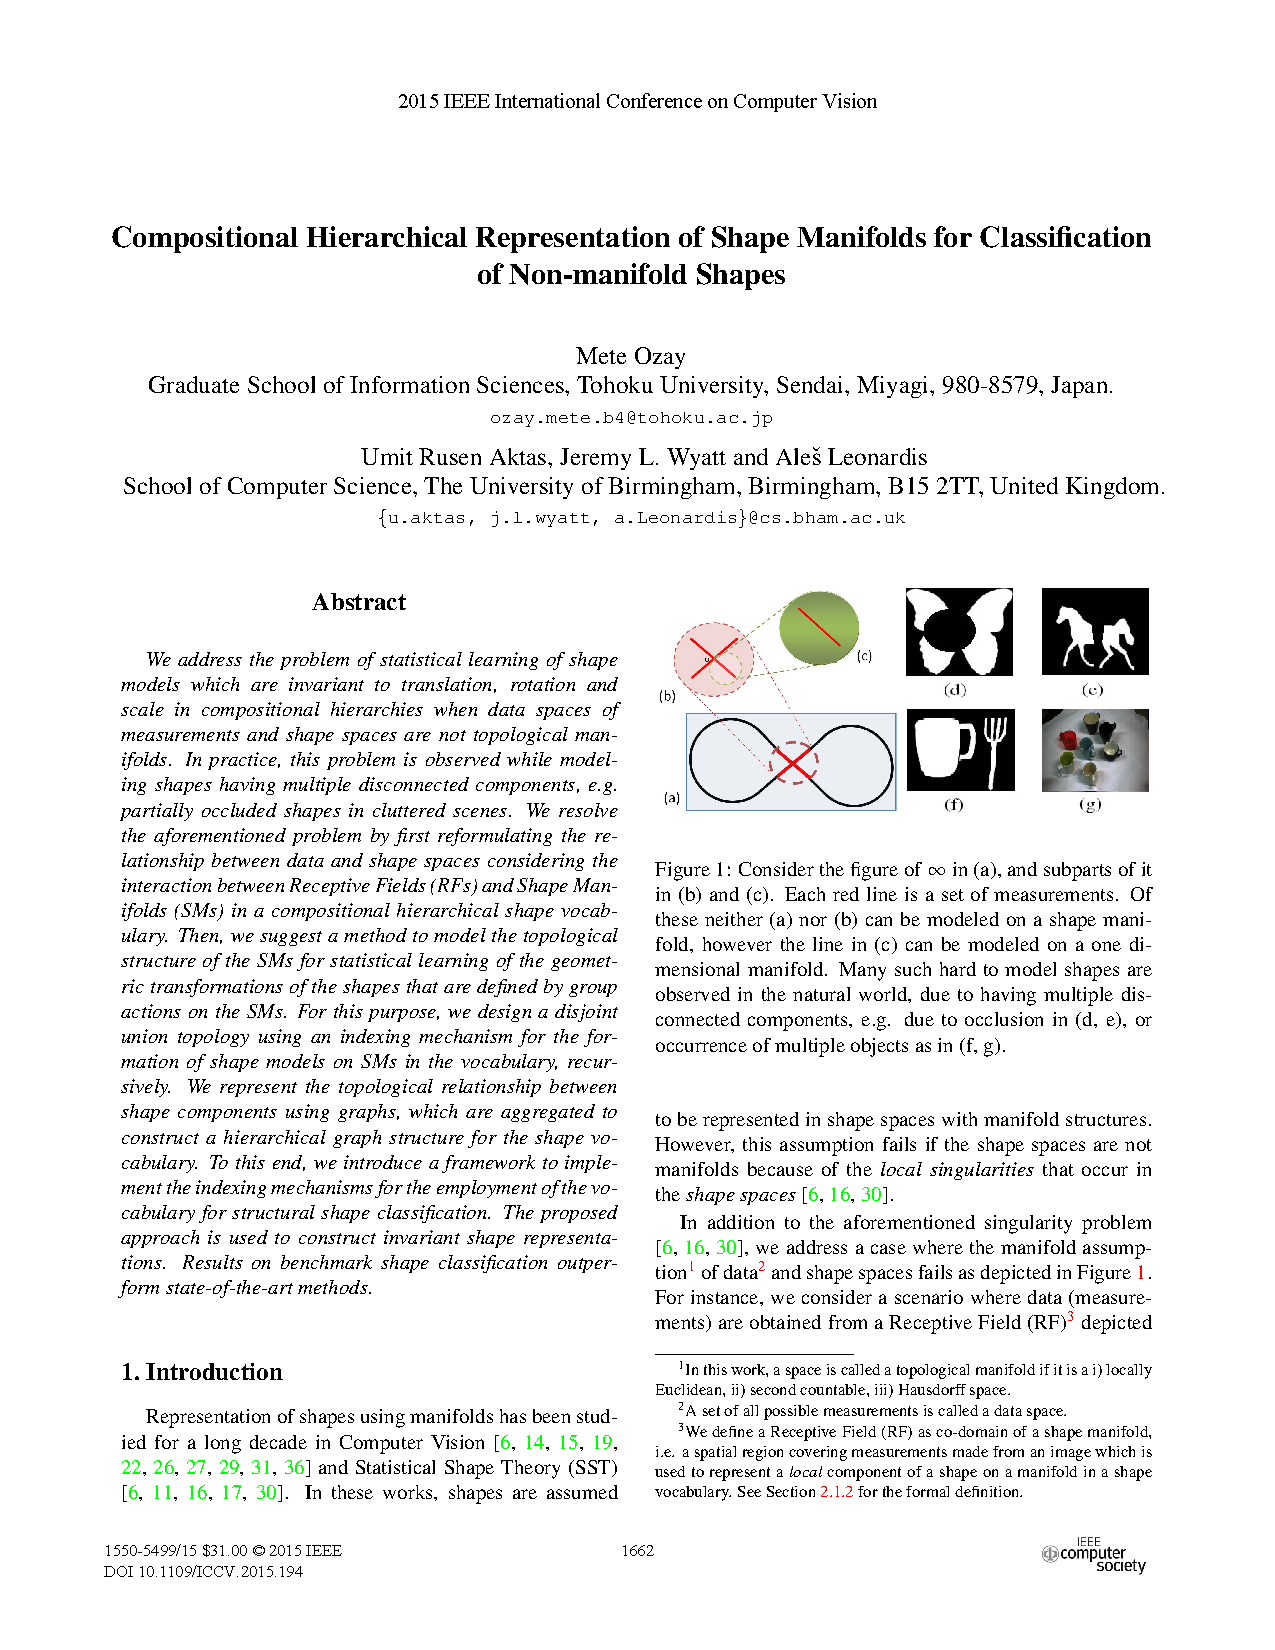
\includepdf[pages=-]{./attachedPapers/Ozay_Compositional_Hierarchical_Representation_ICCV_2015_paper.pdf}

\end{document}
